%%%%%%%%Bilecik �eyh Edebali �niversitesi M�hendsilik Fak�ltesi%%%%
%%%%%%%%%%%Bilgisayar M�hendisli�i Proje I-II �al��mas�%%%%%%%%%%%%
%%%%%%%%%%%%%%%%%%%%%%LaTeX Class%%%%%%%%%%%%%%%%%%%%%%%%%%%%%%%%%%
\documentclass{BUP}
%%%%%%%%%%%%%%%%%%%%%%%%%%%%%%%%%%%%%%%%%%%%%%%%%%%%%%%%%%%%%%%%%%%%%%%%%%%
\begin{document}
\shorthandoff{=}%grafik komutlar�nda babelden kaynaklanan hatay� engeller.
%%%%%%%%%%%%%Proje I-II �al��malar�n�n B�l�mleri%%%%%%%%%%%%%%%%%%%%%%%%%%%
\thispagestyle{empty} %Bu sayfaya sayfa numaralar� yaz�lmaz
\begin{figure}[H]
\centering
\includegraphics[scale=0.2]{logomuz}
%Bu komutla resim dosyam�z� y�kl�yoruz.
\end{figure}
%sa�a 4 sol 2 a�a�� yukar� 3%
\begin{center}
\textbf{T.C.}\\
\textbf{B�LEC�K �EYH EDEBAL� �N�VERS�TES�}\\
\textbf{M�HEND�SL�K FAK�LTES�}

\textbf{B�LG�SAYAR M�HEND�SL��� B�L�M�}
\end{center}

\vspace*{4cm}%bir miktar bo�luk b�rakmak i�in
\begin{center}
\textbf{MOB�L UYGULAMALI EV OTOMASYONU}

\textbf{MEHMET �EL�K}

\textbf{PROJE II �ALI�MASI}
\end{center}

\vspace*{\fill}
\begin{center}
\textbf{PROJE DANI�MANI : Do�. Dr. Emre DANDIL}

\textbf{B�LEC�K}\\ 
\textbf{\today}
\end{center}

\thispagestyle{empty} %Bu sayfaya sayfa numaralar� yaz�lmaz
\begin{figure}[H]
\centering
\includegraphics[scale=0.2]{logomuz}
%Bu komutla resim dosyam�z� y�kl�yoruz.
\end{figure}
%sa�a 4 sol 2 a�a�� yukar� 3%
\begin{center}
\textbf{T.C.}\\
\textbf{B�LEC�K �EYH EDEBAL� �N�VERS�TES�}\\
\textbf{M�HEND�SL�K FAK�LTES�}

\textbf{B�LG�SAYAR M�HEND�SL��� B�L�M�}
\end{center}

\vspace*{4cm}%bir miktar bo�luk b�rakmak i�in
\begin{center}
\textbf{MOB�L UYGULAMALI EV OTOMASYONU}

\textbf{MEHMET �EL�K}

\textbf{PROJE II �ALI�MASI}
\end{center}

\vspace*{\fill}
\begin{center}
\textbf{PROJE DANI�MANI : Do�. Dr. Emre DANDIL}

\textbf{B�LEC�K}\\ 
\textbf{\today}
\end{center}

\pagenumbering{roman}%romen rakamlar� kullan�lmaya ba�lan�yor.
\setcounter{page}{2}% sayfa numaras�n� ii'den ba�lat�l�yor.
\centerline{\bf �ZET}
\addcontentsline{toc}{section}{�ZET}
\begin{center}
\textbf{Projenin Amac�}
\end{center} 
\begin{small}
�e�itli sens�r ve devre elemanlar�n�n birbirleri ile ve mobil uygulama ile anl�k haberle�mesini sa�layarak end�stri 4.0 ile beraber gelen nesnelerin interneti �zerine bir proje geli�tirmektir.
\end{small}

\begin{center}
\textbf{Projenin Kapsam�}
\end{center}
\begin{small}
Projemizde g�stermelik olsa'da bir devre kurulacakt�r. Bu devre bir sunucuya bulundu�u ortamda'ki �s�, nem ve gaz de�erlerini g�nderirken ayn� zamanda s�rekli olarak sunucuda ki verileri okuyacak ve gelen veriye g�re elektrikli sistemlerin kontrol�n� sa�layacakt�r. Ayn� �ekilde mobil uygulamada hem sunucudan gelen de�erleri okuyup-yazacak hemde sunucuya veri g�nderecekdir. B�ylece mobil uygulama ve devre s�rekli olarak haberle�mi� olacakt�r.
\end{small}


%%%%%%%%%%%%%%%%%%%%%%%%%%%%%%%%%%%%%%%ABSTRACT%%%%%%%%%%%%%%%%%%%%%%%%%%%%%%%%%%%%%%%%%%
\newpage
\centerline{\bf ABSTRACT}
\addcontentsline{toc}{section}{ABSTRACT}
\begin{center}
\textbf{Project Objective}
\end{center}


\begin{small}
Developing a project on the IOT that comes with industry 4.0 by providing instant communication of various sensors and circuit elements with each other and with the mobile application.
\end{small}
%Bilecik �eyh Edebali University Department of Computer Engineering students is studied. The aim of project is work to create a template for writing \LaTeX\ writing the final report template in the Project, to be written.

\begin{center}
\textbf{Scope of Project}
\end{center}
\begin{small}
A circuit will be established in our project, even if it is only for show. While this circuit sends the temperature, humidity and gas values of the environment to a server, it will also continuously read the data on the server and control the electrical systems according to the incoming data. Likewise, in the mobile application, it will both read and write the values from the server and send data to the server. Thus, the mobile application and the circuit will be in constant communication.
\end{small}
%Bilecik �eyh Edebali University Computer Engineering Department Bilecik need to create a project template Latex codes assignment, involves the use of. The first part of the project consists of two parts, \LaTeX's development have been studied and why it is preferred that the use of information provided in the information. Faculty of Engineering of the university for the second part, Sheikh Edebali Bilecik Project Paper \LaTeX\ codes and are included.


%As a result, Bilecik Sheikh Edebali University Computer Engineering
%Department prepared a document that students can build project reports into \LaTeX. 
\addcontentsline{toc}{section}{TE�EKK�R}
\section*{TE�EKK�R}
Bu projenin ba��ndan sonuna kadar haz�rlanmas�nda  eme�i bulunan ve 
beni bu konuya y�nlendiren sayg�de�er hocam ve dan��man�m 
Say�n Do�. Dr. Emre DANDIL'a t�m katk�lar�ndan ve hi� 
eksiltmedi�i deste�inden dolay� te�ekk�r ederim.
\vspace{2cm}

\begin{flushright}
\textbf{MEHMET �EL�K}

\today
\end{flushright}
\tableofcontents%bu komutun oldu�u yerde i�indekiler olu�turulur.
\renewcommand*\listfigurename{\centerline{\bf\normalsize �EK�L L�STES�}}
\listoffigures%bu komutun oldu�u yerde �ekiller listesi olu�turulur
\addcontentsline{toc}{section}{�EK�L L�STES�}
\pagenumbering{arabic}%Sayfa numaralamas�n� arap rakamlar�yla yapar.
\setcounter{page}{1}%sayfa numaras�n� 1'den ba�lat�r.
\section{G�R��}
\begin{normalsize}
Evler'de ve Binalar'da i�in ak�ll� kelimesi ilk olarak Amerika Birle�ik Devletlerinde 1980 y�l�n�n ba�lar�nda
kullan�lm��t�r. T�rkiye'deki ilk uygulama ise 1984 y�l�nda yap�lm��t�r. Bu sistem yaln�zca
izlemeye y�nelik olarak tasarlanm��t�r. Ge�en y�llar i�inde teknolojinin geli�mesine paralel
olarak ya�ant�m�z�n her alan�nda ciddi de�i�imler oldu. Mekatronik sistemlerdeki geli�meler
daha h�zl�, daha y�ksek kapasiteli kontrol cihazlar�n�n kullan�lmas�na imk�n verdi[1].

 
Teknoloji geli�tik�e insanlar hayatlar�n� kolayla�t�ran, ihtiya�lar�na
cevap verebilen, kendilerine daha g�venli, daha konforlu ve en �nemlisi daha tasarruflu bir
ya�am sunan sistemlere ihtiyac� artmaktad�r.
Ev teknolojilerinin ki�iye �zel ihtiya� ve isteklere g�re �ekillendirilmesi ile olu�an sisteme ev
otomasyonu denir. Ev otomasyon kontrol� ile evde s�cakl�k kontrol�, ayd�nlatma kontrol�,
g�venlik kontrol�, yang�n alarm
sistemi, vb. ev otomasyonun �al��ma alanlar�ndand�r[2].

G�venlik sistemleri ve otomasyonlar ya�anan bir �ok afet ve h�rs�zl�k olay�n� engelleyebilir. �rne�in T�rkiye'de meydena gelen asayi� olaylar�n�n \%27'si h�rs�zl�k olaylar�d�r. Meydena gelen h�rs�zl�k olaylar�n�n �o�unlu�u ise �ok basit �nlemler al�narak engellenebilir olaylard�r[3]. 

G�n�m�zde en yayg�n ve kullan��l� �nlemler ise ak�ll� ev sistemleridir. Ak�ll� ev sistemlerinde ise en �nemli husulardan biri yang�n ve h�rs�z alarm sistemleridir. ��nk� bu sistemler do�rudan can ve mal g�venli�i ile ilgilidir[4].
\end{normalsize}
\newpage
\section{TEKNOLOJ� GEL���M�}
\begin{normalsize}
�lk olarak geleneksel yap�n�n hakim oldu�u tar�m
d�nemindeki de�i�imin h�z� ile kapitalist sanayi devrimi sonras� modern olarak adland�r�lan d�nemdeki
de�i�imin h�z� birbirinden �ok farkl�d�r.
ilk olarak, yakla��k 1100 y�l �nce avc� toplay�c� d�nemden yerle�ik hayata ge�i�e imkan veren neolitik devrim ya�anm��t�r ve sanayi devriminin ger�ekle�ti�i 18.yy'�n sonuna kadar s�rm��t�r. Bu uzun tar�m d�nemi boyunca insanlar ihtiya�lar�n� topraktan kar��lam��lard�r. �retimi ba�latmak i�in gerekli olan �ey toprakt�r.
Tar�m d�nemi boyunca insanlar�n tar�msal �retimde
kulland�klar� ara�lar�n/aletlerin sanayi devrimine kadar �ok b�y�k bir farkl�l�k g�stermedi�i g�r�l�r. Bu
d�nemde orak, �eki�, saban, t�rpan gibi el aletleri tar�mda yayg�n olarak kullan�lm�� ve uzun tar�m d�nemi boyunca bu aletlerde b�y�k bir bi�imsel de�i�im
olmam��t�r. De�i�im daha �ok aletlerin yap�m�nda
kullan�lan hammaddede (ta�, maden vs.) g�r�l�r.
1700'l� y�llar�n sonuna gelindi�inde ise yeni enerji t�r� olan su ve buhar teknolojisi ile sanayi devrimi ba�layacakt�r. Bu devrim ile birlikte tar�msal faaliyeti yapma
bi�imimiz dahil de�i�im t�m
alanlarda g�r�lecek ve hissedilecektir. Burada yap�sal bir d�n���m ya�anarak sanayi devrimi ger�ekle�ir[5].

\end{normalsize}
\subsection{End�stri 4.0}
\begin{normalsize}
End�stri 4.0 ya da d�rd�nc� sanayi devrimi olarak bilinen bu s�re�, son �retim teknolojilerinin, otomasyon sistemlerinin
ve bu sistemi olu�turan teknolojilerinin bir birleriyle veri al��veri�inde bulundu�u sistemi ifade etmektedir. Bu yeni sistem,
Siber G�venlik, Siber-Fiziksel Sistemler, Bulut Teknolojileri, Ak�ll� Fabrikalar, Nesnelerin �nterneti, �nternet Servisleri,
��renen Robotlar, B�y�k Veri, Sanal Ger�eklik ve 3 Boyutlu Yaz�c�lar gibi y�ksek teknoloji i�erikli bile�enlerden
olu�maktad�r[6].
�lk kez 2011 y�l�nda Almanya'daki Hannover Fuar�'nda duyuran End�stri 4.0, son zamanlarda d�nya
�ap�nda akademisyenler, uygulay�c�lar, politikac�lar ve h�k�met yetkilileri taraf�ndan s�rekli dikkate al�nan
bir konu olmu�tur. Kagermann (2013), End�stri 4.0 kavram�n� �retim teknolojilerinde otomasyon ve veri
transferine y�nelik yeni bir trend olarak tan�mlamaktad�r. 

\end{normalsize}

\subsection{T�rkiye'de End�stri 4.0}
\begin{normalsize}

D�rd�nc� end�stri devriminin geli�mekte oldu�u son y�llarda teknolojinin kullan�labilirli�i
konusunda T�rkiye'nin g�stergeleri �ok �nemlidir. T�rkiye Jeopolitik co�rafyas� nedeniyle geli�mekte
olan devrimin transferi noktas�nda Avrupa ve Asya aras�nda �nemli bir k�pr�d�r. Bu devrimin �nc�l���n� yapan Alman firmalar�n�n T�rkiye'deki fabrikalar�nda ArGe �al��malar�na h�z verdikleri
bilinmektedir. Bu firmalarla rekabet edebilecek olan yerli firmalar�nda bundan sonraki stratejileri �nem
kazanm��t�r.
2020 y�l�nda 14 milyar cihaz�n bir birine ba�lanabilir olaca�� hedefi �l�� al�n�rsa T�rkiye'de
ileti�im alt yap�s�n�n geni�letilmesi gerekebilir. T�rkiyede Bilgisayar kullan�m� \%95,9 , �nternet eri�imi \%93,7 gibi y�ksek rakamlara ula�sa da web sitesi sahipli�i \%66 seviyesindedir.
D�rd�nc� sanayi devriminin ileti�imde ve ula��mda h�z �a��n� ya�att���n� d���nd���m�zde
giri�imcilerin internet �zerinden �retim ve pazarlama a�lar�n� geni�letmesi i�in web sitesi sahipli�inin
giderek artan bir seyirde olmas� gerekti�i d���n�lebilir. Cihazlar�n, robotlar ve nesnelerin interneti ile birbirine ba�lanaca��n�, ak�ll� fabrikalar�n
kurulaca��n� dikkate ald���m�zda ayr�ca bu fabrikalar�n otomasyonlar arac�l���yla y�netilip web siteleri
arac�l��� ile uygulamalar �zerinden de y�netilece�ini g�z �n�ne ald���m�zda, giri�imlerde internet ve
web sitesi sahipli�i konusunda hen�z yeterli donan�ma sahip olmad���m�z s�ylenebilir[7].
\end{normalsize}

\subsection{Nesnelerin �nterneti}
\begin{normalsize}
Internet kullan�m�n�n insanlar aras�ndaki ileti�imi, bilgi payla��m�n� ve kar��l�kl� etkile�imi artt�rarak
g�nl�k hayat�m�z� �nemli �l��de de�i�tirdi�i art�k ka��n�lmaz bir ger�ektir. Nesnelerin interneti olarak adland�r�lan yeni teknolojik kavram ak�ll� cihazlar�n, birbirlerini alg�layan ve
ileti�ime ge�ebilen nesneler arac�l���yla ak�ll� ba�lant�s� �eklinde tan�mlanmaktad�r. Bu teknoloji ile �ok
say�da, k���k boyutlu, kablosuz teknoloji kullanabilen alg�lay�c� (sensor) cihazlar ile ya�ad���m�z
�evredeki (ev, okul, i�yeri, fabrika, �ehir vb.) hemen hemen b�t�n olaylar� izlemek ve bilgi toplamak
m�mk�nd�r. Ayn� �ekilde �retim/imalat ile ilgili end�striyel sistemlerden aktar�labilecek gerekli
verileri de Bilgi Sistemi i�inde kullanabilmek End�striyel IoT (IIoT) olarak isimlendirilen bir di�er
kavram� ortaya ��karm��t�r. Ortamdaki alg�lay�c� cihazlardan ve �retimdeki veri terminallerinden gelen,
ger�ek zamanl� s�rekli veri ak���, internet ortam�nda Bulut Servis Sa�lay�c�lar taraf�ndan verilen
depolama, veritaban�, uygulama hizmetleri ile Bilgi Sistemleri taraf�ndan kullan�lmaya haz�r hale
getirilmektedir. B�yle bir IIoT bilgi ak��� g�nl�k ya�ant�m�z�, i� hayat�n� ve end�striyel �retim
sistemlerini olumlu y�nde etkileyebilecek de�i�ikliklere neden olacakt�r. End�stri ve IoT'nin
birle�tirilmesi ile �retimde kullan�lan ak�ll� cihazlar, insan hatas�n� en aza indirerek, ger�ek zamanl�
bilginin karar destek sistemleri taraf�ndan de�erlendirilmesini sa�layacakt�r. Bu da �retimde kalitenin
artt�r�lmas�, maliyetlerin azalt�lmas�, rekabet�i �r�nler yarat�lmas� gibi bir�ok olumlu etki yaratacakt�r.
Bu �al��mada Nesnelerin �nterneti'nin end�striyel �retime uyarlanmas� ile ilgili �al��malar incelenmi�,
otomatik depolama, �nleyici bak�m, madencilik, ak�ll� �evre d�zenlemeleri gibi farkl� uygulama
�rneklerinde IoT'nin yaratt��� olumlu katk�lar tart���lm�� ve geli�meye a��k hususlar hakk�nda bilgi
verilmi�tir[8].
\end{normalsize}
\newpage
\section{DONANIM VE YAZILIM ALTYAPISI}
\begin{normalsize}
Proje ayn� anda bir IOT projesi, ev otomasyonu ve g�venlik sistemi olacakt�r. Kurdu�um devrede kullan�lan sens�r ve bile�enler g�stermelik olmakla beraber sistem bir evin t�m elektronik e�yalar�n�n kontrol�n� sa�layabilir. Daha �ok ve geli�mi� sens�rler ile �al��abilmektedir.


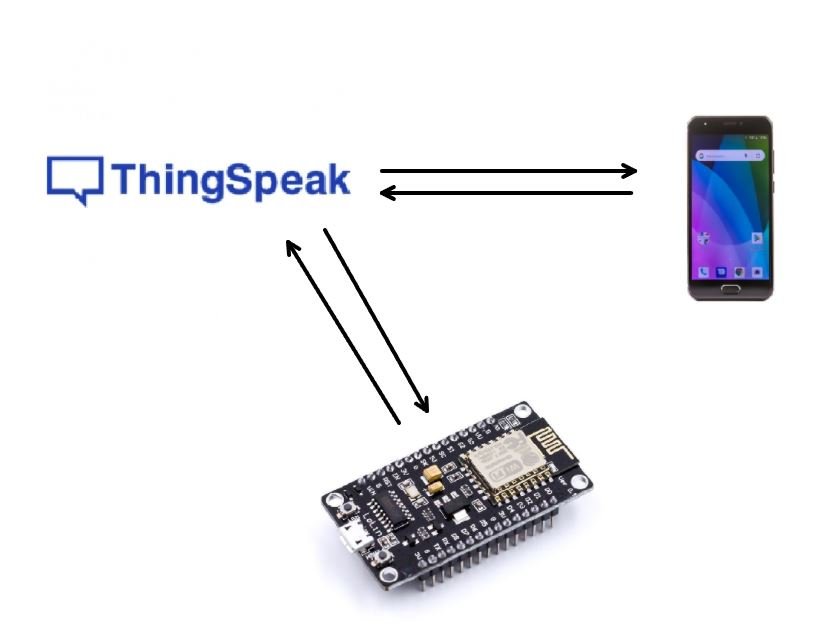
\includegraphics[scale=0.45]{1}
\begin{figure}[!ht]
    \centering    
  
    \caption{IoT �rne�i}
     \label{fig:res1}
\end{figure}

�ekilde 1 g�r�ld��� �zere kurulan g�stermelik sens�rler �s�,nem,gaz bilgilerini devremiz bir sunucuya g�nderecek. Sunucu ise bu bilgileri mobil uygulamaya g�nderecek. Led,lamba vb. kontrollerini sa�larken de mobil uygulama sunucuya veri yollayacak. devremiz ise sunucuda ki gerekli bilgileri anl�k okumaya devam edecek gelen veriye g�re lamba, led kontrol� ger�ekle�ecek.
\end{normalsize}
\subsection{Haberle�me}
\begin{normalsize}
Sunucu olarak proje'de ThingSpeak kullan�lacakt�r. ThingSpeak �cretsiz bir IOT geli�tirme sistemi bize sunar. �cretsiz s�r�m� 8 adet �zerine veri yazabile�imiz ve veri okuyabilece�imiz label sunuyor. 

\newpage
\begin{figure}[!ht]
    \centering    
  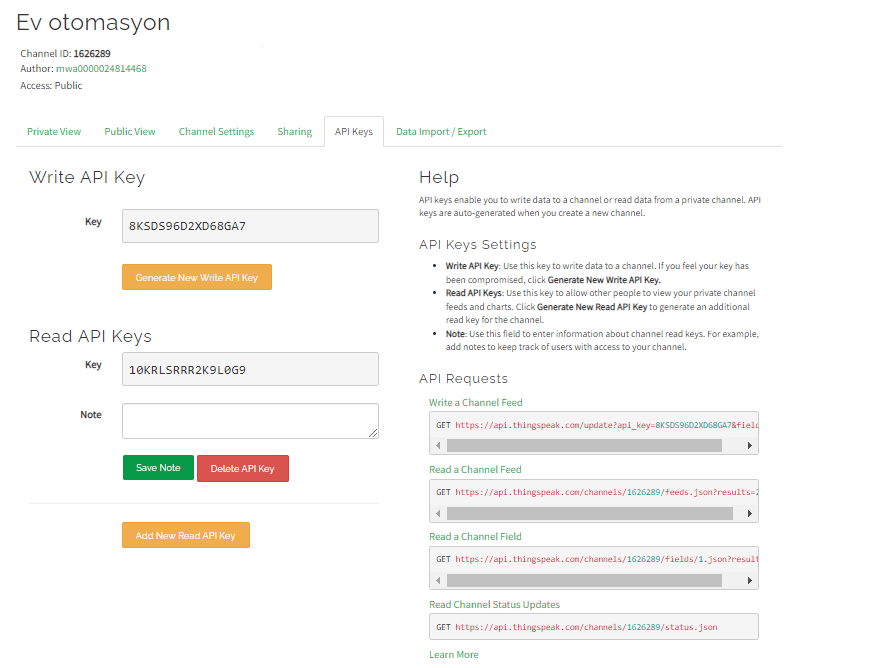
\includegraphics[scale=0.4]{8}
    \caption{ThingSpeak logosu}
     \label{fig:res1}
\end{figure}
Kullan�m kolayl��� ve �cretsiz olmas� sayesinde pop�ler ve sevilen bir sistem olsada veri yazma ve okuma h�z� olduk�a d���k. G�nderilen bir veriyi 30 saniye ile 2 dakika aras�nda al�yor. Bu durumsa en �ok led vb kontrollerinde sorun ��kart�yorq . 
�ekil 2 thingspeak �zerinde veri yazma okuma i�in verilen keyler.

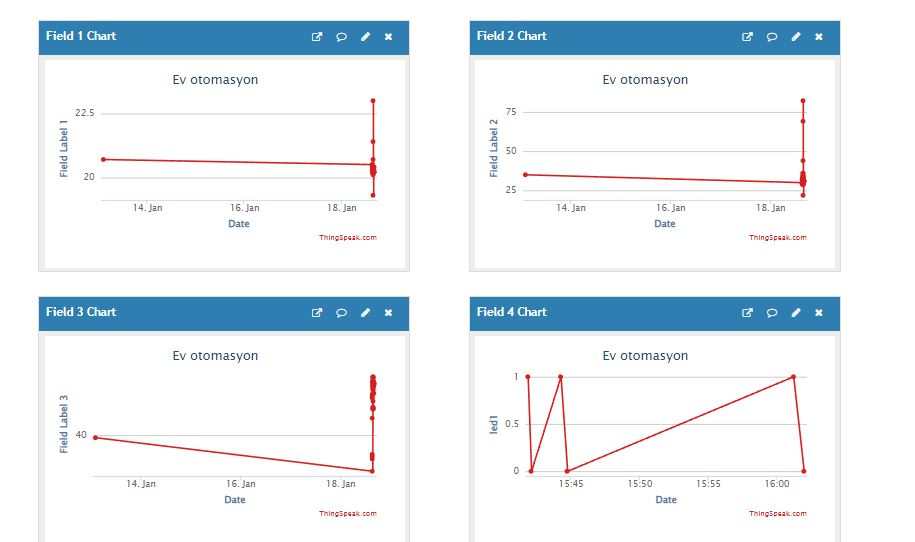
\includegraphics[scale=0.5]{7}
\begin{figure}[!ht]
    \centering    
  
    \caption{ThingSpeak tablosu}
     \label{fig:res1}
\end{figure}
\end{normalsize}

�rnek olarak �ekil 3 gibi thingspeak sitesi �zerinden verilerimizi tablo olarak g�rebiliyoruz. �ekilde �s�,nem,led lambalar�n durumunu grafik olarak g�rebiliyoruz fakat bizim projemizde bu tablolara ihtiyac�m�z yok ve kullanmayaca��z.
\newpage
\subsection{Mobil Uygulama}



\begin{normalsize}

Son y�llarda mobil cihazlar hayat�m�za b�y�k
�l��de y�n vermeye ba�lam��t�r. �lk
zamanlarda sadece telefon g�r��mesi ve k�sa
mesaj g�nderimi gibi fonksiyonlar� i�eren bu
cihazlar g�n�m�zde b�y�k bir de�i�im
s�recine girmi�tir. Mobil cihazlar aras�nda
ak�ll� telefonlar (smartphone) art�k bir
bilgisayardan farks�z bir hale gelmi� olmakla
birlikte, her �l�ekteki i�letmeler taraf�ndan
artan oranlarda bir�ok faaliyetin
y�r�t�lmesinde kullan�lmaktad�r[9].

Teknolojinin h�zl� geli�iminden belki de en b�y�k pay� alan
ak�ll� telefon ve tabletler gibi kablosuz ileti�im olana�� sa�layan cihazlar�n daha iyi, h�zl� ve
ucuz modellerle herkesin zorlanmadan ula�abilece�i bir konuma gelmesi sebebiyle d�nya
�ap�nda mobil cihazlar b�y�k kitleler taraf�ndan benimsenmeye ba�lanm��t�r[10].

Projemizde bir mobil uygulamada olacak. Mobil uygulama ile s�cakl�k,nem,gaz durumunu g�r�t�lerken lamba ve led kontrol� yapabilece�iz. Mobil uygulamam�z Unity isimli bir oyun motoru ile yap�lacak.
Unity bir �ok farkl� ortamda ��kt� alabilece�iniz bir oyun motorudur. Kolay kullan�m�,
basit aray�z�, geni� e�itim ve asset materyali bulma olas�l��� ve en �ok'ta �cretsiz olmas� bu kadar pop�ler olmas�n� sa�lam��t�r.

Unity oyun motoru, Danimarka'da Unity Technologies taraf�ndan geli�tirilmi� bir
oyun motorudur. Unity, �zel i�leme motorunu ile nVidia PhysX fizik motoruyla b�t�nle�tirir
Microsoft'un a��k kaynak uygulamas� .NET kitapl�klar� ile kullan�labilmesi
unity'i pop�ler hale getirmi�tir[11].
Unity aslen bir oyun motoru olmas�na kar��n bu tip mobil uygulamalar geli�tirmek ve mobil uygulamalar�n ��kt�s�n� almak i�in kolayl�klar sa�lar.

\begin{figure}[!ht]
    \centering    
  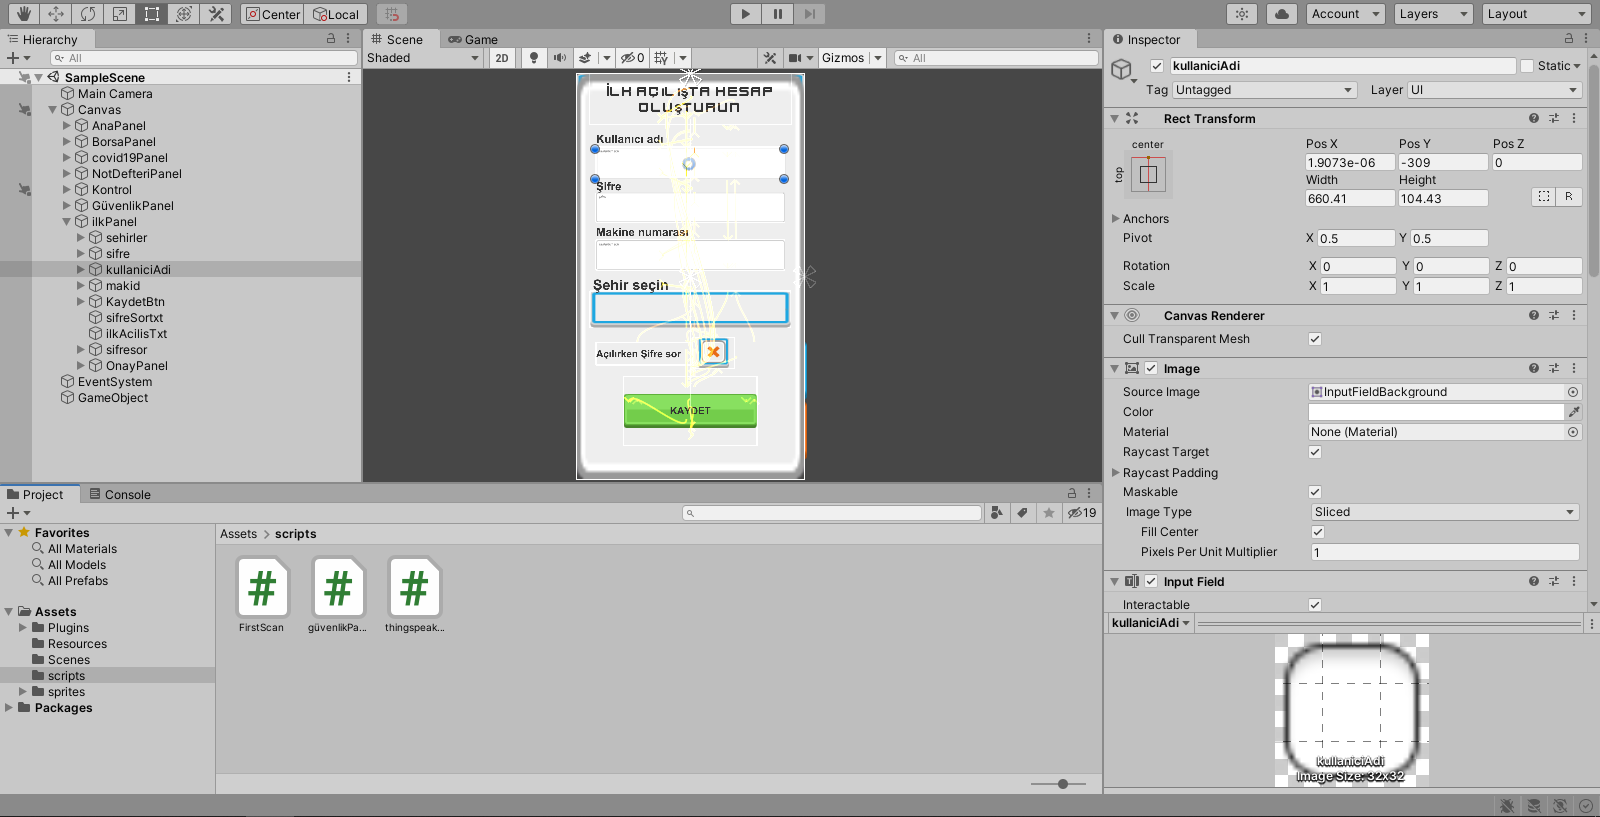
\includegraphics[scale=0.35]{unity}
    \caption{Unity aray�z�}
     \label{fig:res1}
\end{figure}
\newpage
Unity aray�z� �ekil 4'te g�r�ld��� �zere bir oyun motoruna k�yasla sadece bir aray�ze sahiptir. Bu k�s�mda geli�tirici oyun objelerini kontrol etti�i "hierarchy" panelini, oyun i�i yerle�imi kontrol etti�i "scane" panelini, oyunun en son halini g�rd��� "game" paneli, oyun i�i dosyalar i�in "project" paneli ve se�ili objenin �zelliklerini g�steren "Inspector" paneli bulunur.
\begin{figure}[!ht]
    \centering    
  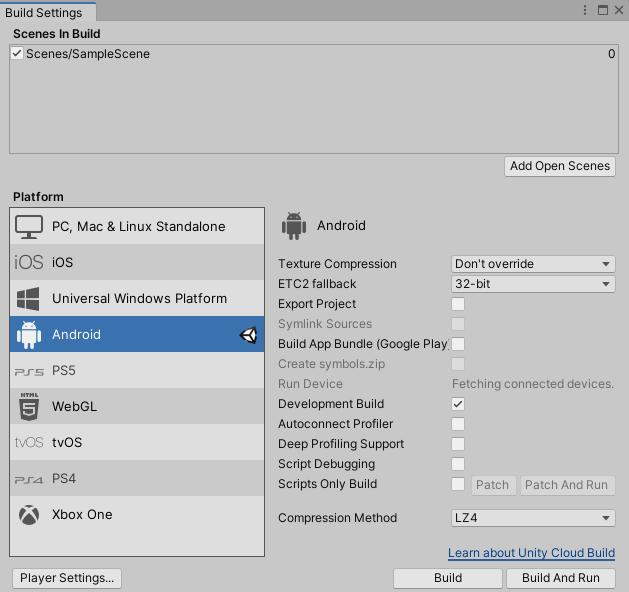
\includegraphics[scale=0.4]{build}
    \caption{Unity build aray�z�}
     \label{fig:res1}
\end{figure}

�ekil 5 Unity build aray�z�nde g�r�ld��� �zere Unity bir �ok farkl� plartforma �ok kolay bir �ekilde ��kt� almam�z� sa�lar. 
\end{normalsize}
\newpage
\begin{figure}[h!]
    \centering    
  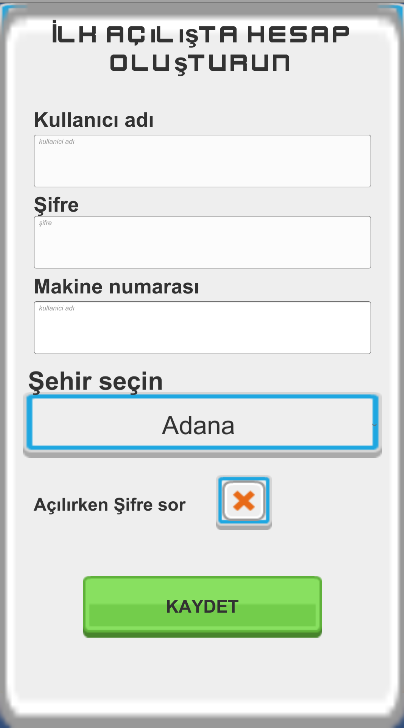
\includegraphics[scale=0.55]{ev1}
    \caption{Hesap olu�turma}
     \label{fig:res1}
\end{figure}

E�er uygulama ilk defa a��l�yor ise �ekil 6'da g�r�len panel a��lacak ve bir hesap olu�turman�z� isteyecek. Kullan�c�dan kullan�c� ad� ve �ifre istenecek. Kullan�c�n�n istedi�ine g�re her a��l��ta �ifre sorulacak veya sorulmayacak.
Ayr�ca kullan�c�dan �ehir bilgisi istenecek. Bu bilgi ile hangi �ehrin hava durumu bilgilerini se�ece�imizi belirleyece�iz.
Son olarak kullan�c�dan bir makine numaras� alaca��z. Bu makine numaras� devremizin ba�l� oldu�u thingspeak kanal�n�n id numaras� olacak. B�ylece farkl� cihazlar ile uygulamam�z sadece id numaras� de�i�tirilip kullan�labilir olacak.

\newpage
\begin{figure}[h!]
    \centering    
  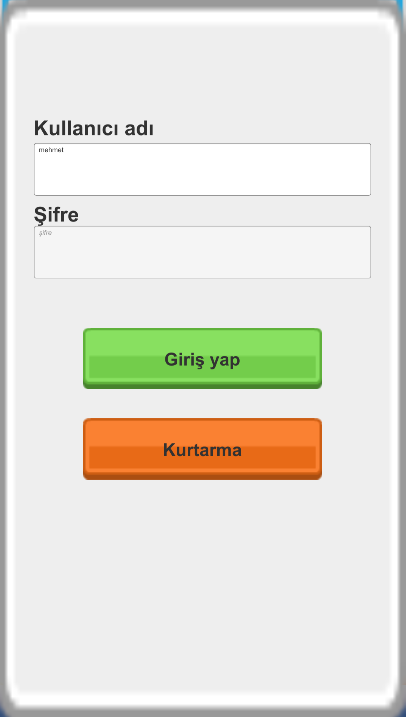
\includegraphics[scale=0.4]{ev2}
    \caption{G�venlik paneli}
     \label{fig:res1}
\end{figure}

Kullan�c� istedi�ine g�re her a��l��ta �ekil 7 g�venlik paneli ��kacak. Do�ru bilgeleri giremedi�imiz s�rece hata verecek.
�ifre ve kullan�c� ad� unutulursa kurtarma se�ene�i olacak fakat bu t�m kaydedilmi� veriyi silecek ve yeni bir hesap olu�turma zorunda kal�nacak.

\begin{figure}[h!]
    \centering    
  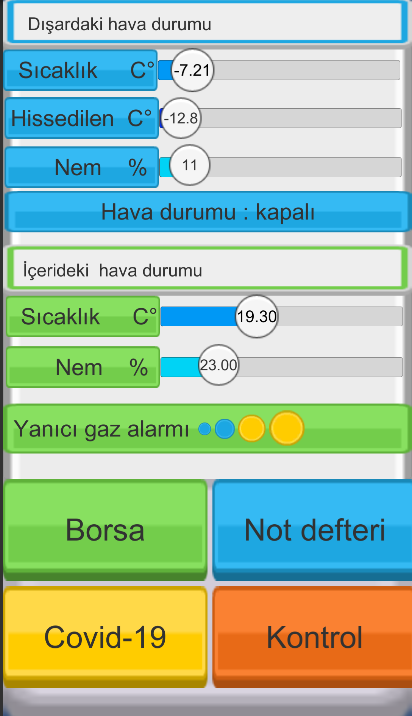
\includegraphics[scale=0.4]{ev3}
    \caption{Ana panel}
     \label{fig:res1}
\end{figure}

Girilen bilgiler do�ru ise �ekil 8 ana panele ula�m�� olunacak.
\newpage
\begin{figure}[h!]
    \centering    
  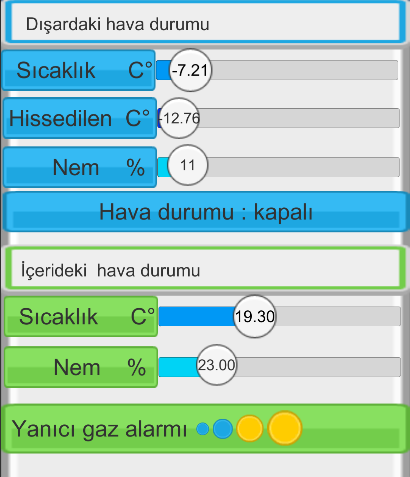
\includegraphics[scale=0.5]{cek}
    \caption{Ana panel verileri}
     \label{fig:res1}
\end{figure}

Ana panelde �ekil 9'da g�r�ld��� �zere d��ar�daki hava durumunu ve i�erdeki hava durumunu g�rebiliyoruz. 
D��ardaki hava durumunu weather api �zerinden �ekerken i�erideki yani devremizin oldu�u yerdeki hava durumunu de�erlerini ise thingspeak �zerinden �ekiyoruz.
Altta ise di�er panellere ula�abilece�imiz 4 adet buton bulunuyor.

\begin{figure}[h!]
    \centering    
  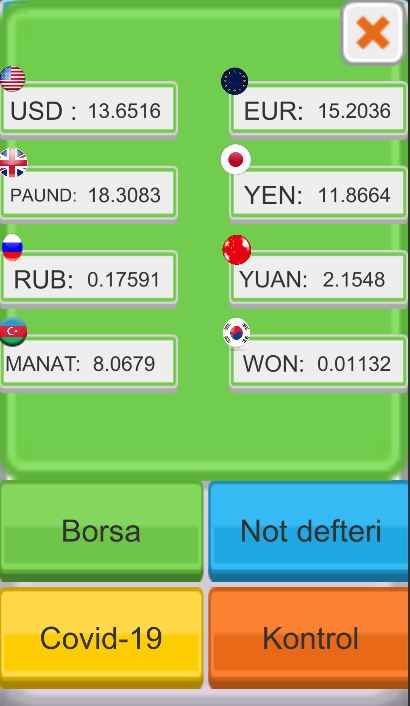
\includegraphics[scale=0.5]{ev4}
    \caption{Borsa paneli}
     \label{fig:res1}
\end{figure}

Yukar�da �ekil 10'da g�r�ld��� �zere uygulama da �zerinden g�ncel d�viz kurlar�n� g�r�nt�lenir.
\newpage
\begin{figure}[h!]
    \centering    
  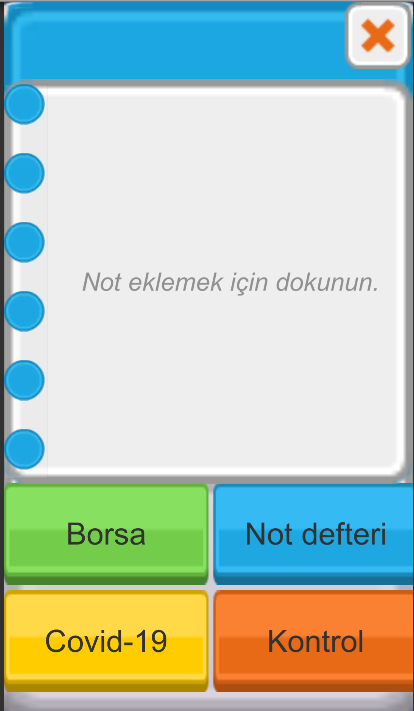
\includegraphics[scale=0.45]{ev5}
    \caption{Not tutma paneli}
     \label{fig:res1}
\end{figure}

�ekil 11 not tutma panelinde ise ihtiyaca g�re not tutabilinir. Girilen notlar kaydedilir sonra yine ayn� panelden d�zenlenebilir veya eklenebilir.

\begin{figure}[h!]
    \centering    
  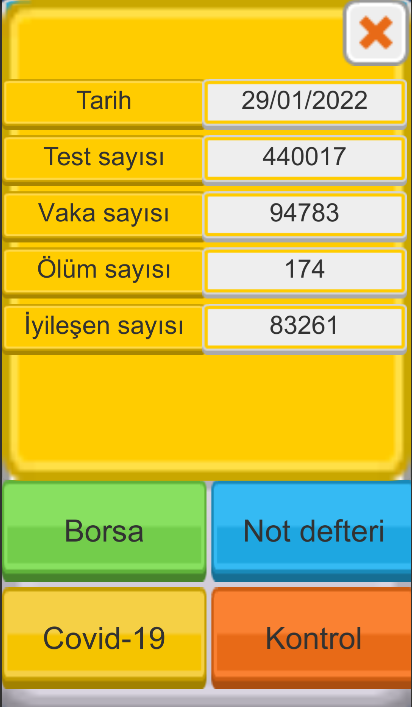
\includegraphics[scale=0.45]{ev6}
    \caption{Covid-19 paneli}
     \label{fig:res1}
\end{figure}

�ekil 12 Covid-19 panelinde ise sa�l�k bakanl��� taraf�ndan g�nl�k g�ncellenen Covid-19 verilerini g�r�nt�lenebilir.

\newpage
\begin{figure}[h!]
    \centering    
  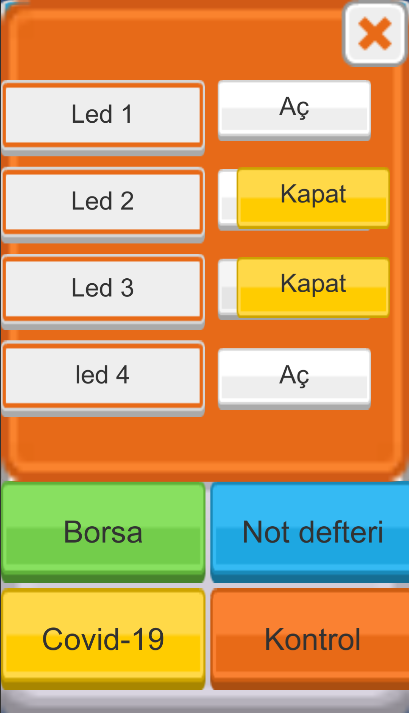
\includegraphics[scale=0.45]{ev7}
    \caption{Elektrik kontrol paneli}
     \label{fig:res1}
\end{figure}
Thingspeak sunucusuna veri g�ndererek ve devremiz ile gelen veriyi okuyarak tamamen internet �zerinden ba�ka herhangibi ba�lant� olmadan led kontrol� sa�lanmantad�r. Normalde thingspeak sunucusu kendini 30 saniye ile 2 dakika aras�nda g�nceller. Bu sorun ledlerin anl�k yan�p s�nmesine engeller. Fakat sunucuya veri yazarken veri yaz�lmaz ise sunucunun geri 0 d�nd�rd���n� e�er veri yaz�l�rsa ise ka��nc� yaz�lan veri oldu�una g�re 1 veya daha y�ksek bir say� d�nd�r�r. Bu sayede led a� butonuna t�klad���m�z zaman led yanana kadar sunucuya veri g�nderebiliriz. Led yand���nda ise uygulamada ledi kapat butonu gelmektedir.

\newpage
\subsection{Mobil Uygulama Kodlar�}
Uygulama genel olarak veri okumaya veya veri yazmaya dayal�. �ncelikle g�venlik panelleri ve ve a��l�� ekran� kontrollerini yapan kodlar ile ba�layal�m.
\begin{figure}[h!]
    \centering    
  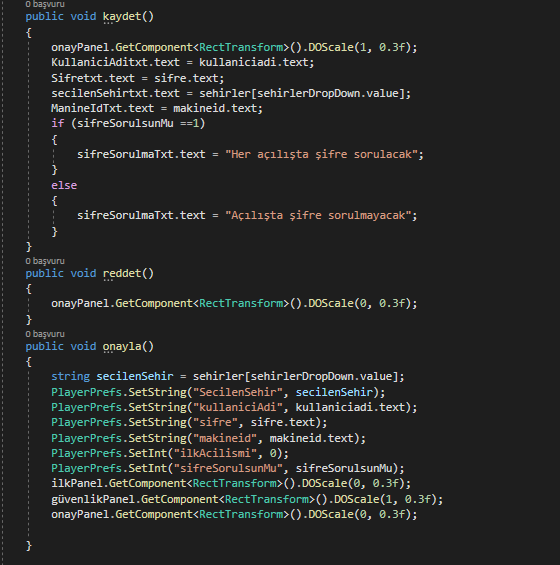
\includegraphics[scale=0.6]{kodlar1}
  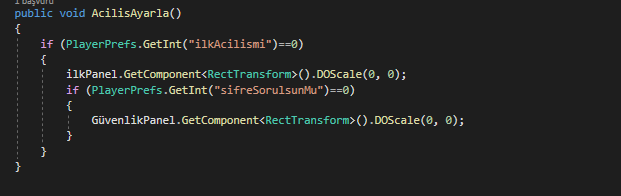
\includegraphics[scale=0.7]{kodlar3}
    \caption{G�venlik ve a��l�� kontrol kodlar�}
     \label{fig:res1}
\end{figure}

\begin{normalsize}
�ekil 14'de kodlar'da daha �ok unity'nin sa�lad��� kolayl�klardan yararlanarak kullan�c�dan ald���m�z verileri yerel bir dosyaya kaydetmi� oluyoruz. Ayr�ca dotween plugin ile panel kontrolleri sa�l�yoruz. �rnek vermek gerekirse :
\textbf{"PlayerPrefs.SetString("isim", "Mehmet");"} Bu kod ile yerel kal�c� haf�zada isim ad�nda i�inde Mehmet yazan string bir ifadeyi tutulur. "Set" yerine "Get" yazarakda �a�r�labilir.                  
\textbf{"g�venlikPanel.GetComponent
<RectTransform>().DOScale(1, 0.3f);"} Bu ifade ile unity �zerinde g�venlik paneli olarak belirlenen oyun objesine ait scale de�erini 1 yapar ve bunu 0.3 saniyelik zamanda yapar. B�yleyece panel kapan�rken animasyonlu gibi kapanm�� olur. 
\end{normalsize}
\newpage
\begin{figure}[h!]
    \centering    
  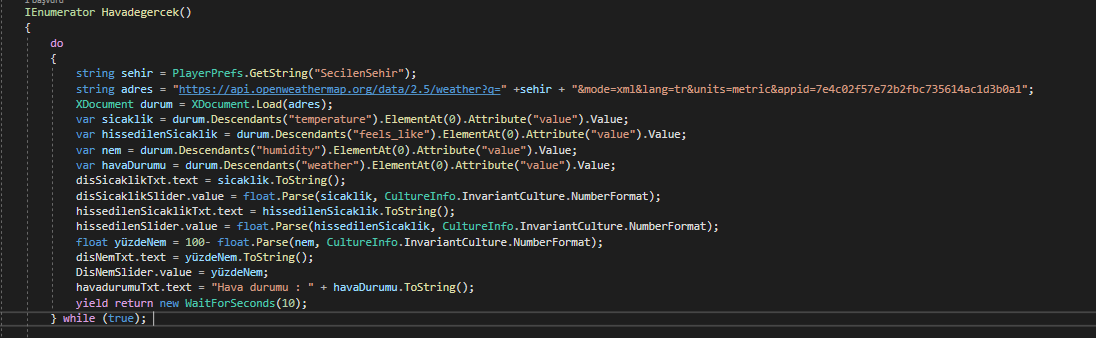
\includegraphics[scale=0.55]{kodlar4}
    \caption{Hava durumu bilgisi kodlar�}
     \label{fig:res1}
\end{figure}

�ekil 15'te weather api'nin bize vermi� oldu�u token ile d��ar�da ki hava durumunu �ekiyoruz. G�r�ld��� �zere xml �zerinden kodu �ekiyoruz. Kullan�c�dan ald���m�z �ehir bilgisine g�re kodu �ekiyor. �ekti�i verileri ana panelde(�ekil 7-8) slider ve text objelerine yazd�r�yoruz. Unity'nin sa�lad��� avantajlardan biri olan bir kod ile "yield return new WaitForSeconds(10);" ile bu i�lem her 10 saniyede 1 defa tekrar ediyor. Bu metod C++ da olan delay metodu ile ayn� mant�kta �al���r. 
\begin{figure}[h!]
    \centering    
  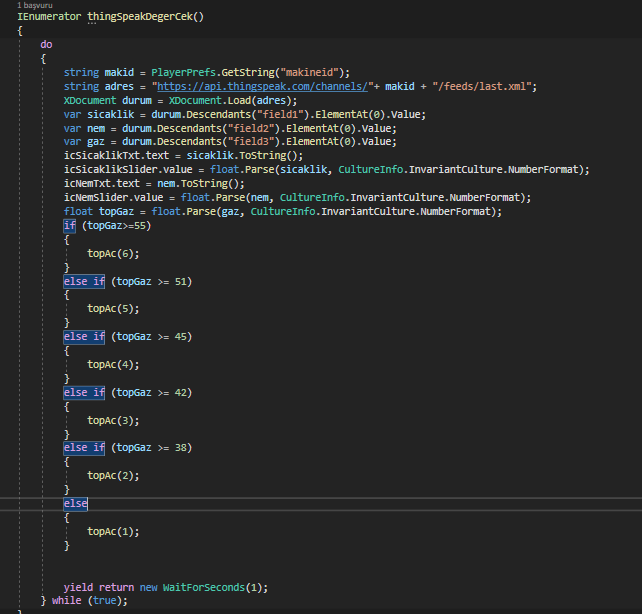
\includegraphics[scale=0.5]{kodlar5}
    \caption{Thingspeakden veri �ekme kodlar�}
     \label{fig:res1}
\end{figure}

�ekil 16'te thingspeakden �zerinden yine xml formatta olan verileri benzer �ekilde �ekiyoruz. Benzer �ekilde borsa ve covid-19 verilerine de �ekilir.
\newpage
\begin{figure}[h!]
    \centering    
  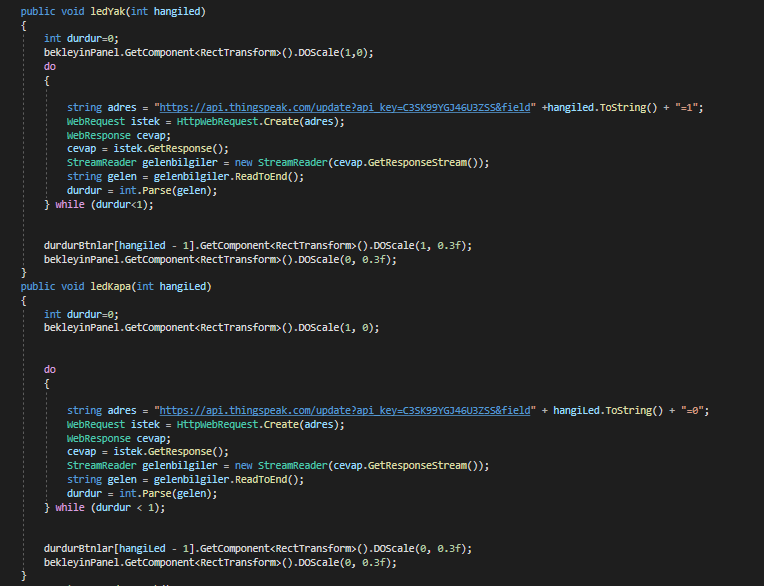
\includegraphics[scale=0.7]{kodlar6}
    \caption{Thingspeakden veri yazma kodlar�}
     \label{fig:res1}
\end{figure}
�ekil 17'ta unity'de belirledi�imiz buton numaras�n� d��ardan alan bir void ile thingspeak'in bize verdi�i yaz komutunu web iste�i olarak yolluyoruz. Sonra sitenin bize geri d�nd�rd��� yan�t� al�p bak�yoruz. Site 0'dan daha b�y�k bir yan�t �evirene kadar i�lem devam ediyor. Thingspeak'de sunucu dolu oldu�u zamanlar veri yazm�yor. Yazmas� sunucu durumuna ba�l� olarak 30 saniye ile 2 dakika aras� al�yor. E�er sunucu veriyi almazsa 0 geri d�nd�r�yor. Al�rsa ise ka��nc� yaz�lan veri oldu�una g�re 1 veya daha y�ksek bir say� �eviriyor. Bizim kodumuzda ise sunucu 1 veya daha fazla say� �evirene kadar while d�ng�s� devam ediyor.






\subsection{Elektronik Devre}
\begin{normalsize}
Projede g�stermelikte olsa bir devre haz�rlasam'da proje asl�nda �ap� �ok daha b�y�kt�r. Bir evde ki t�m g�venlik sistemlerini, t�m cihazlar�, t�m elektrik devrelerinin kontrol� online ortamda ger�ekle�tirilebilir.

Projemizde bir adet mikroi�lemci olacak. Mikrodenetleyici veya mikroi�lemciler, herhangi bir �evre birimini veya donan�m� y�netmeyi sa�layan basit
bilgisayarlard�r. Mikrodenetleyiciler programlanarak uzaktan veya direk ba�lant� ile makinalar�
y�netmeye, veri almaya, kontrol etmeye olanak sa�layan, i�erisinde bir haf�za birimi, i�lemci ve
giri�/��k�� birimleri bar�nd�ran cihazlard�r[12].


\begin{figure}[h!]
    \centering    
  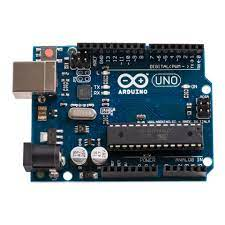
\includegraphics[scale=0.8]{6}
    \caption{Ardiuno uno}
     \label{fig:res1}
\end{figure}
Arduino Uno (�ekil 18), �talyan m�hendislerin geli�tirmi� oldu�u a��k kaynak yaz�l�ml� ve donan�ml�,
�zerinde ATmega328 mikrodenetleyicisinin bulundu�u bir elektronik geli�tirme kart�d�r. Arduino 14 tane dijital, 6 tane analog giri� ve ��k��lara, 32KB Flash belle�e ve 16 MHZ
h�z�nda a��k kaynak donan�ma sahiptir. Arduino i�erisindeki bootloader program� ile programlanmas� i�in harici bir programa gerek
duymamaktad�r. Java platformunda geli�tirilen Arduino IDE Kod edit�r�, Wiring programlama dili ile C
ve C++ tabanl� k�t�phanelerini kontrol kart�na y�klemekte kullan�lmaktad�r. Arduino donan�m
�zelliklerine g�re, Due, Uno, Mega, LillyPad, Esplora,Pro Mini,Mini, Nano, BT, Fio �e�itlenmektedir[13].

Bu projede ardiuno ile yap�labilen her �eyi yapabildi�imiz nodemcu'yu kullanaca��z(�ekil 19). Nodemcu i�inde esp8266 mikroi�lemcisi olan nodemcu ayr�ca dahili �ekilde i�inde gelen wifi mod�l� ile internete ba�lanmam�z� sa�layacak.

\newpage
\begin{figure}[h!]
    \centering    
  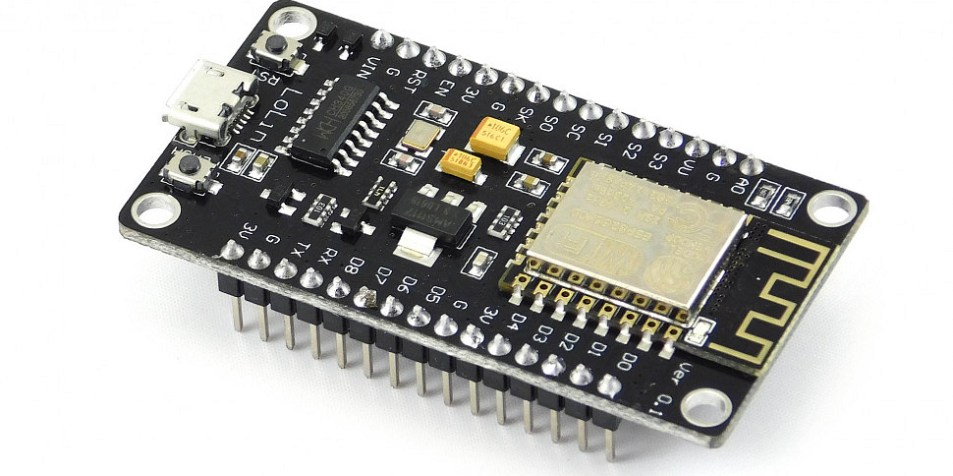
\includegraphics[scale=0.3]{esp}
    \caption{Nodemcu esp8266}
     \label{fig:res1}
\end{figure}

\end{normalsize}

\begin{normalsize}
Devrede(�ekil 20) kullan�lacak devre elemanlar�.
\begin{itemize}
\item 1 adet nodemcu lolin esp8266 mikrodenetleyicisi.
\item 1 adet mq2 gaz sens�r�.
\item 1 adet dht11 s�cakl�k ve nem sens�r�.
\item 1 adet buzzer.
\item 1 adet hc sr04 ultrasonik mesafe sens�r�.
\item 4 adet led.
\item breadboard, jumper koblolar, diren�ler.
\end{itemize}

\begin{figure}[h!]
    \centering    
  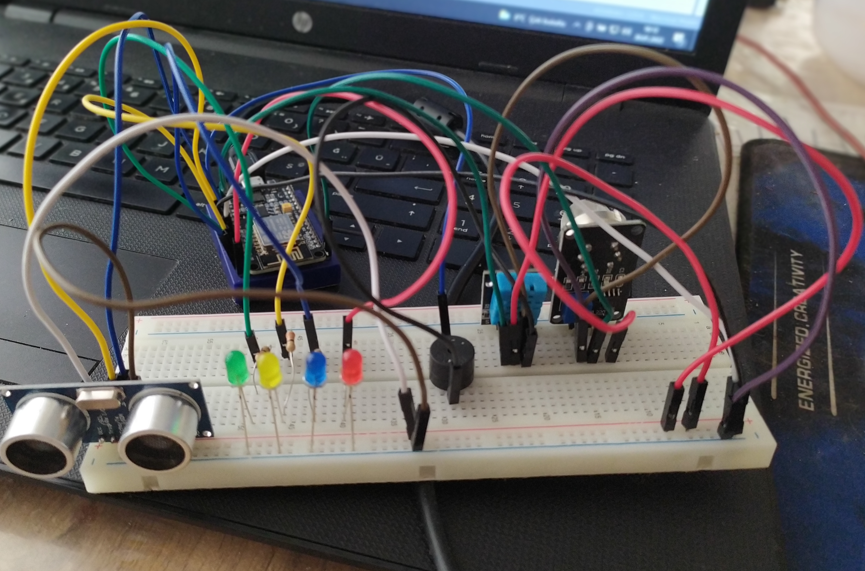
\includegraphics[scale=0.4]{devree}
    \caption{Devre}
     \label{fig:res1}
\end{figure}
\end{normalsize}
\newpage
\begin{figure}[h!]
    \centering    
  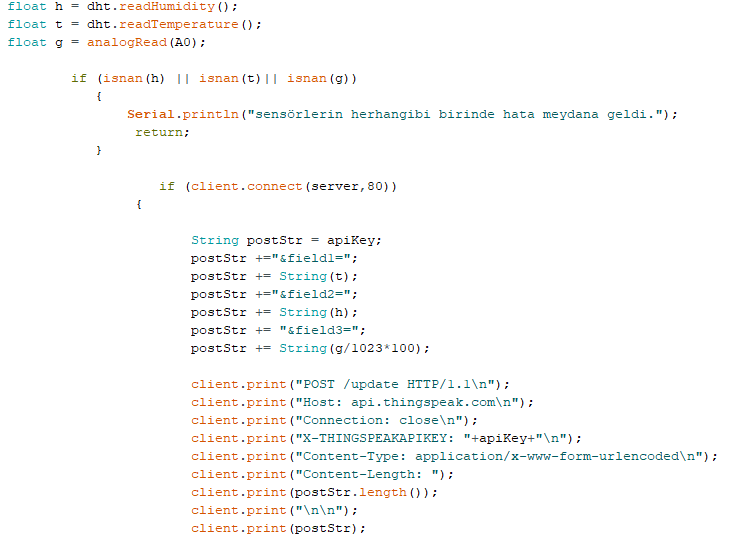
\includegraphics[scale=0.7]{kodlar7}
    \caption{Dht11 ve mq2 sens�r kodlar�}
     \label{fig:res1}
\end{figure}

Ba�lad���m�z dht11 ve mq2 sens�rlerinden gelen veriyi okuyor ve thingspeak �zerine yaz�yoruz(�ekil 21).

\begin{figure}[h!]
    \centering    
  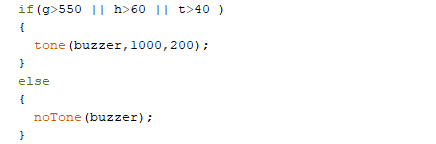
\includegraphics[scale=0.8]{kodlar8}
   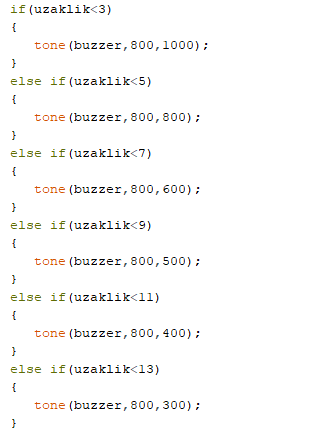
\includegraphics[scale=0.5]{kodlar9}
    \caption{Buzzer kodlar�}
     \label{fig:res1}
\end{figure}

De�erler a��r� y�ksek gelirse buzzer �al���yor ve alarm veriyor.
sens�r devreye yakla��l�nca buzzer �al���yor ve alarm veriyor(�ekil 22).

\newpage

\begin{figure}[h!]
    \centering    
  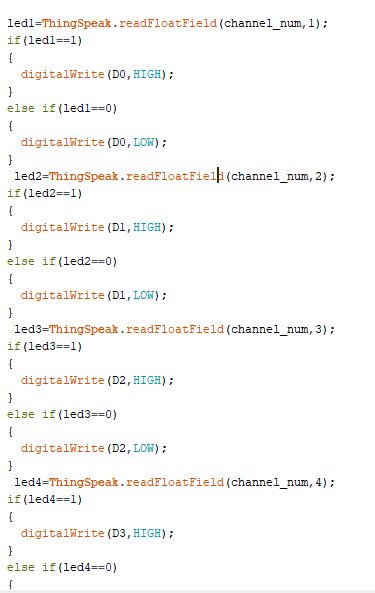
\includegraphics[scale=0.8]{kodlar10}
    \caption{Thingspeak kodlar�}
     \label{fig:res1}
\end{figure}

Thingspeak k�t�phanesi ile bu sefer devremiz veri okuyor. Uygulamadan yollad���m�z verilere g�re ledler a��p, kapatabiliyor(�ekil 23).
















\section{SONU�LAR VE �NER�LER}
\begin{normalsize}
G�n ge�tik�e cihazlar internet �zerinden kontrol edilebilir ve birbirleri ile ileti�im halinde �al��maya ba�layacaklar. �leride tamamen internet �zerinden kontrol edilen ve i�inde ki t�m cihazlar�n birbirleri ile ba�lant�l� �al��an otomasyonlar yap�lacak gibi g�r�n�yor. Bu sayede insanlar insalar�n i� hayat�, g�venli�i, vb. durumlar �ok daha iyi hale getirilebilir. Bu durum avantajlar�n�n yan�nda dezavantajlar getirebilir. Gizlilik sorunlar�, siber sald�r�lar gibi. Yinede gelecekte nesnelerin interneti kelimesi �ok daha fazla duyulan bir kelime olmas� kesin gibi.

Bu projede ise bu t�r otomasyonlar�n k���k bir similasyonu yap�lmaya �al���lm��t�r. Yapt���m�z mobil uygulama ve devre s�rekli birbiri ile ileti�im halinde kal�yor. Birbirleri ile s�rekli veri al��veri�i yap�yor. Bu sisteme daha geli�mi� cihazlar tak�labilir. Evde ki t�m cihazlar(Buzdolablar�, �ama��r makineleri, Su �s�t�c�lar�, lambalar vb.) birbireleri ile ileti�im halinde �al��abilir. Uygulama �zerinden evde hangi cihazlar�n aktif hangilerinin pasif oldu�u g�r�lebilir. Yine internet �zerinden bu cihazlar kapat�labilir veya a��labilir.

\end{normalsize}
\section{EKLER}
\textbf{Kaynak kodlar icin github profilim github.com/MehmetCelik07}



\renewcommand{\refname}{KAYNAKLAR}
\addcontentsline{toc}{section}{KAYNAKLAR}
\begin{thebibliography}{99}%kaynak ortam� olu�turmak i�in
%%%%Kaynak Web sayfas�ndan al�nm�� ise%%%%%%%%%%%%%%%%%
\bibitem{k:1} Yumurtac�, Mehmet, and Ali Ke�eba�. "AKILLI EV TEKNOLOJ�LER� VE OTOMASYON S�STEMLER� SMART BUILDING TECHNOLOGIES AND ITS AUTOMATION SYSTEMS." (2009).
\bibitem{k:2} Kongaz, Hande. "Ak�ll� ev otomasyonun mikrodenetleyici ile ger�ekle�tirilmesi." (2007). 
\bibitem{k:3} Polat, C. , Eren, H. , Erbak�c�, F. "HIRSIZLIK SU�UNU ETK�LEYEN FAKT�RLER�N DE�ERLEND�R�LMES� VE GELECE�E Y�NEL�K YAKLA�IMLAR" . G�venlik Bilimleri Dergisi 2 (2016 ): 1-34 <https://dergipark.org.tr/en/pub/gbd/article/239719>
\bibitem{k:4} Y�lmaz, C. , G�rdal, O. "Bilgisayar Kontroll� Bir Bina Otomasyonunun Tasar�m� ve Uygulamas�" . Politeknik Dergisi 9 (2006 ): 241-246 <https://dergipark.org.tr/en/pub/politeknik/issue/33023/367121>
\bibitem{k:5} Aksoy, Suat. "De�i�en teknolojiler ve end�stri 4.0: end�stri 4.0'� anlamaya dair bir giri�." SAV Katk� 4 (2017): 34-44.
\bibitem{k:6} AKBEN, ��r �yesi �brahim, and ��r G�r �lker �brahim AV�AR. "END�STR� 4.0 VE KARANLIK �RET�M: GENEL B�R BAKI�." T�rk Sosyal Bilimler Ara�t�rmalar� Dergisi 3.1 (2018): 26-37.
\bibitem{k:7} Bulut, Ela, and Taner AK�ACI. "End�stri 4.0 ve inovasyon g�stergeleri kapsaminda t�rkiye analizi." ASSAM Uluslararas� Hakemli Dergi 4.7 (2017): 55-77.
\bibitem{k:8} Ercan, Tuncay, and Mahir Kutay. "End�stride nesnelerin interneti (IoT) uygulamalar�." Afyon Kocatepe �niversitesi Fen ve M�hendislik Bilimleri Dergisi 16.3 (2016): 599-607.
\bibitem{k:9} Ada, Serkan, and H. Tatl�. "Ak�ll� telefon kullan�m�n� etkileyen fakt�rler �zerine bir ara�t�rma." K. Mara� S�t�� �mam �niversitesi, �� BF, ��letme B�l�m�, Kahramanmara� (2012).
\bibitem{k:10} Keskin, Nilg�n �zdamar, and Ara� G�r Hakan KILIN�. "Mobil ��renme uygulamalar�na y�nelik geli�tirme platformlar�n�n kar��la�t�r�lmas� ve �rnek uygulamalar." A��k��retim Uygulamalar� ve Ara�t�rmalar� Dergisi 1.3 (2015): 68-90.
\bibitem{k:11} Craighead, Jeff, Jennifer Burke, and Robin Murphy. "Using the unity game engine to develop sarge: a case study." Proceedings of the 2008 Simulation Workshop at the International Conference on Intelligent Robots and Systems(IROS 2008). 2008.
\bibitem{k:12}BA���FT��, Fatih, and Kamil Aykutalp G�ND�Z. "NESNELER�N �NTERNET� UYUMLU M�KRODENETLEY�C�LER �ZER�NE B�R ARA�TIRMA." Sel�uk �niversitesi Sosyal ve Teknik Ara�t�rmalar Dergisi 18 (2019): 62-71.
\bibitem{k:13} S�ZEN, Ahmet Ali, et al. "Arduino Kontroll� �izim Robotu." Mehmet Akif Ersoy �niversitesi Fen Bilimleri Enstit�s� Dergisi 8.�zel (Special) 1 (2017): 79-87.



\end{thebibliography}
\centerline{\textbf{�ZGE�M��}}
\addcontentsline{toc}{section}{�ZGE�M��}
\begin{table}[H]
{
\renewcommand{\arraystretch}{1.5}
\begin{tabular}{l@{\bf :}l}
\multicolumn{2}{l}{\underline{\bf K���SEL B�LG�LER}}\cr
\textbf{Ad� Soyad�}& \; Mehmet �elik    \cr
\textbf{Uyru�u}&\; T�rk  \cr
\textbf{Do�um Yeri ve Tarihi}&\; Antalya/Manavgat 09.02.1999     \cr
\textbf{Adres}&\;   Be�ikta� Mahallesi, Ulutepe Sokak, No:40 Bilecik/Merkez   \cr
\multicolumn{1}{l}{}&      \cr
\textbf{Telefon}&\; 0 545 952 59 78    \cr
\textbf{e-mail}&\; mehmethancelik077@gmail.com  \cr
\multicolumn{1}{l}{}&\cr
\multicolumn{2}{l}{\underline{\bf E��T�M DURUMU}}\cr
\textbf{Lisans ��renimi}&\; B�E� Bilgisayar M�hendisli�i B�l�m�\cr
\textbf{Bitirme Y�l�}&\; Devam   \cr
\textbf{Lise}& \;  Manavgat Teknik ve Meslek Anadolu Lisesi  \cr
\multicolumn{1}{l}{}&\cr
\multicolumn{2}{l}{\underline{\bf �� DENEY�MLER�}}\cr
\textbf{Y�l}&\;     \cr
\textbf{Kurum}& \;    \cr
\textbf{Stajlar}&\;     \cr
\multicolumn{1}{l}{}&\cr
\multicolumn{2}{l}{\underline{\bf �LG� ALANLARI:}}\cr
\multicolumn{1}{l}{}&\cr
\multicolumn{2}{l}{\underline{\bf YABANCI D�LLER:}}\cr
\multicolumn{1}{l}{}&\cr
\multicolumn{2}{l}{\underline{\bf BEL�RTMEK �STED���N�Z D��ER �ZELL�KLER:}}
\end{tabular}}
\end{table}
\shorthandon{=}
\end{document}
%%%%%%%%%%%%%%%%%%%%%%%%%%%B�TT�%%%%%%%%%%%%%%%%%%%%%%%%%%%%%%%%%%%%%%%%%%%%%
